% J. Musilová a P. Musilová, Matematika I: pro porozumnění i praxi: netradiční
% výklad tradičních témat vysokoškolské matematiky. VUTIUM, 2009, s. 339, isbn:
% 978-80-214-3631-2. WWW: http://localhost/stable.php?id=527 
% https://1drv.ms/b/s!Ajq2sO-eH2xU9XEhAGXpHPItEUvR
% https://tex.stackexchange.com/questions/247541/

\documentclass[11pt, border=2pt]{standalone}
  \usepackage{pgf,tikz,pgfplots}
    \pgfplotsset{compat=1.15}
    \usetikzlibrary{arrows}
    \usetikzlibrary{calc}
    \usetikzlibrary{intersections}
  \usepackage{amsmath}

    \begin{document}
        \definecolor{blue}{rgb}{0,0,1}
        \definecolor{red}{rgb}{0.8,0,0}
        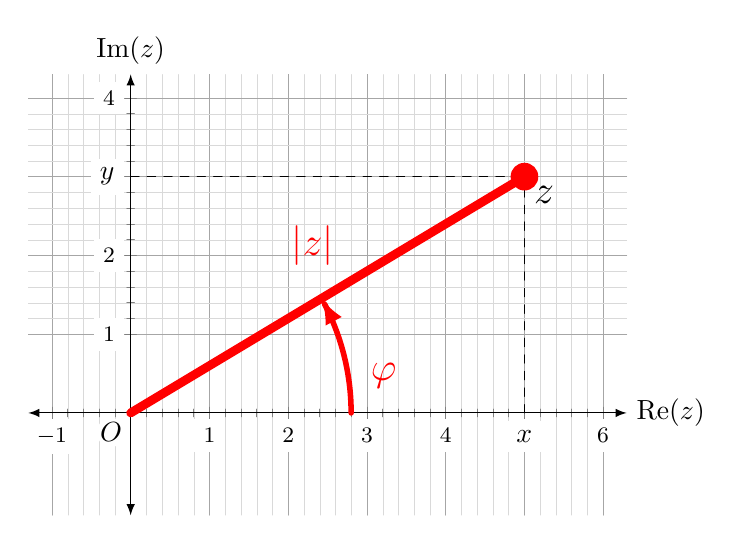
\begin{tikzpicture}[line cap=round,line join=round,>=triangle 45,x=1cm,y=1cm]
            \begin{axis}[
                x=1cm, 
                y=1cm,
                axis lines=middle,
                ymajorgrids=true,
                xmajorgrids=true,
                xmin=-1.1,
                xmax=6.1,
                ymin=-1.1,
                ymax=4.1,
                xtick={-1,0,1,...,6},
                ytick={1,2,...,4},
                grid=both,
                grid style={line width=.1pt, draw=gray!30},
                major grid style={line width=.2pt,draw=gray!70},
                minor tick num=4,
                xlabel style={at={(ticklabel* cs:1)},anchor=west},
                ylabel style={at={(ticklabel* cs:1)},anchor=south},
                ticklabel style={font=\footnotesize,fill=white},
                axis line style={latex-latex},
                xlabel={$\operatorname{Re}(z)$},
                ylabel={$\operatorname{Im}(z)$},
                enlargelimits={abs=0.2}
            ]
            \coordinate (O) at (0,0);
            \node[fill=white,circle,inner sep=0pt] (O-label) at ($(O)+(-135:10pt)$) {$O$};
            
            \draw [line cap=round, line width=3.2pt,color=red]  (0,0) -- (5,3);
            \draw [-latex, name path=myline, shift={(-1.3,-1.1)},line width=2pt,color=red]  
                plot[domain=0:0.5,variable=\t]({1*3*cos(\t r)+0*3*sin(\t r)},{0*3*cos(\t r)+1*3*sin(\t r)});
            \draw (5,+3) node[anchor=north west] {\Large$z$};
            \draw (3.5,+0.75) node[anchor=north east, color=red] {\Large$\varphi$};
            \draw (2.7,+2.5) node[anchor=north east, color=red] {\Large$|z|$};

            \draw[dashed] (0,3) coordinate (a_1) -- (5,3) coordinate (a_2);
            \draw[dashed] (5,0) coordinate (b_1) -- (5,3) coordinate (b_2);
            % and store the coordinate in c.
            \coordinate (c) at (intersection of a_1--a_2 and b_1--b_2);
            \fill[red] (c) circle (5pt);
            \draw (-0.3,+3) node[fill=white] {\(y\)};
            \draw (5,-0.3) node[fill=white] {\(x\)};
            \end{axis}
        \end{tikzpicture}
    \end{document}